%!TEX root = ../blob1.tex

\section{TQFTs via fields}
\label{sec:fields}
\label{sec:tqftsviafields}

In this section we review the construction of TQFTs from fields and local relations.
For more details see \cite{kw:tqft}.
For our purposes, a TQFT is {\it defined} to be something which arises
from this construction.
This is an alternative to the more common definition of a TQFT
as a functor on cobordism categories satisfying various conditions.
A fully local (``down to points") version of the cobordism-functor TQFT definition
should be equivalent to the fields-and-local-relations definition.

A system of fields is very closely related to an $n$-category.
In one direction, Example \ref{ex:traditional-n-categories(fields)}
shows how to construct a system of fields from a (traditional) $n$-category.
We do this in detail for $n=1,2$ (\S\ref{sec:example:traditional-n-categories(fields)}) 
and more informally for general $n$.
In the other direction, 
our preferred definition of an $n$-category in \S\ref{sec:ncats} is essentially
just a system of fields restricted to balls of dimensions 0 through $n$;
one could call this the ``local" part of a system of fields.

Since this section is intended primarily to motivate
the blob complex construction of \S\ref{sec:blob-definition}, 
we suppress some technical details.
In \S\ref{sec:ncats} the analogous details are treated more carefully.

\medskip

We only consider compact manifolds, so if $Y \sub X$ is a closed codimension 0
submanifold of $X$, then $X \setmin Y$ implicitly means the closure
$\overline{X \setmin Y}$.


\subsection{Systems of fields}
\label{ss:syst-o-fields}

Let $\cM_k$ denote the category with objects 
unoriented PL manifolds of dimension
$k$ and morphisms homeomorphisms.
(We could equally well work with a different category of manifolds ---
oriented, topological, smooth, spin, etc. --- but for simplicity we
will stick with unoriented PL.)

Fix a symmetric monoidal category $\cS$.
Fields on $n$-manifolds will be enriched over $\cS$.
Good examples to keep in mind are $\cS = \Set$ or $\cS = \Vect$.
The presentation here requires that the objects of $\cS$ have an underlying set, 
but this could probably be avoided if desired.

A $n$-dimensional {\it system of fields} in $\cS$
is a collection of functors $\cC_k : \cM_k \to \Set$ for $0 \leq k \leq n$
together with some additional data and satisfying some additional conditions, all specified below.

Before finishing the definition of fields, we give two motivating examples of systems of fields.

\begin{example}
\label{ex:maps-to-a-space(fields)}
Fix a target space $T$, and let $\cC(X)$ be the set of continuous maps
from $X$ to $T$.
\end{example}

\begin{example}
\label{ex:traditional-n-categories(fields)}
Fix an $n$-category $C$, and let $\cC(X)$ be 
the set of embedded cell complexes in $X$ with codimension-$j$ cells labeled by
$j$-morphisms of $C$.
One can think of such embedded cell complexes as dual to pasting diagrams for $C$.
This is described in more detail in \S \ref{sec:example:traditional-n-categories(fields)}.
\end{example}

Now for the rest of the definition of system of fields.
(Readers desiring a more precise definition should refer to \S\ref{ss:n-cat-def}
and replace $k$-balls with $k$-manifolds.)
\begin{enumerate}
\item There are boundary restriction maps $\cC_k(X) \to \cC_{k-1}(\bd X)$, 
and these maps comprise a natural
transformation between the functors $\cC_k$ and $\cC_{k-1}\circ\bd$.
For $c \in \cC_{k-1}(\bd X)$, we will denote by $\cC_k(X; c)$ the subset of 
$\cC(X)$ which restricts to $c$.
In this context, we will call $c$ a boundary condition.
\item The subset $\cC_n(X;c)$ of top-dimensional fields 
with a given boundary condition is an object in our symmetric monoidal category $\cS$.
(This condition is of course trivial when $\cS = \Set$.) 
If the objects are sets with extra structure (e.g. $\cS = \Vect$ or $\Kom$), 
then this extra structure is considered part of the definition of $\cC_n$.
Any maps mentioned below between fields on $n$-manifolds must be morphisms in $\cS$.
\item $\cC_k$ is compatible with the symmetric monoidal
structures on $\cM_k$, $\Set$ and $\cS$: $\cC_k(X \du W) \cong \cC_k(X)\times \cC_k(W)$,
compatibly with homeomorphisms and restriction to boundary.
We will call the projections $\cC(X_1 \du X_2) \to \cC(X_i)$
restriction maps.
\item Gluing without corners.
Let $\bd X = Y \du Y \du W$, where $Y$ and $W$ are closed $k{-}1$-manifolds.
Let $X\sgl$ denote $X$ glued to itself along the two copies of $Y$.
Using the boundary restriction and disjoint union
maps, we get two maps $\cC_k(X) \to \cC(Y)$, corresponding to the two
copies of $Y$ in $\bd X$.
Let $\Eq_Y(\cC_k(X))$ denote the equalizer of these two maps.
Then (here's the axiom/definition part) there is an injective ``gluing" map
\[
	\Eq_Y(\cC_k(X)) \hookrightarrow \cC_k(X\sgl) ,
\]
and this gluing map is compatible with all of the above structure (actions
of homeomorphisms, boundary restrictions, disjoint union).
Furthermore, up to homeomorphisms of $X\sgl$ isotopic to the identity 
and collaring maps,
the gluing map is surjective.
We say that fields on $X\sgl$ in the image of the gluing map
are transverse to $Y$ or splittable along $Y$.
\item Gluing with corners.
Let $\bd X = (Y \du Y) \cup W$, where the two copies of $Y$ 
are disjoint from each other and $\bd(Y\du Y) = \bd W$.
Let $X\sgl$ denote $X$ glued to itself along the two copies of $Y$
(Figure \ref{fig:gluing-with-corners}).
\begin{figure}[t]
\begin{center}
\begin{tikzpicture}

\node(A) at (-4,0) {
\begin{tikzpicture}[scale=.8, fill=blue!15!white]
\filldraw[line width=1.5pt] (-.4,1) .. controls +(-1,-.1) and +(-1,0) .. (0,-1)
		.. controls +(1,0) and +(1,-.1) .. (.4,1) -- (.4,3)
		.. controls +(3,-.4) and +(3,0) .. (0,-3)
		.. controls +(-3,0) and +(-3,-.1) .. (-.4,3) -- cycle;
\node at (0,-2) {$X$};
\node (W) at (-2.7,-2) {$W$};
\node (Y1) at (-1.2,3.5) {$Y$};
\node (Y2) at (1.4,3.5) {$Y$};
\node[outer sep=2.3] (y1e) at (-.4,2) {};
\node[outer sep=2.3] (y2e) at (.4,2) {};
\node (we1) at (-2.2,-1.1) {};
\node (we2) at (-.6,-.7) {};
\draw[->] (Y1) -- (y1e);
\draw[->] (Y2) -- (y2e);
\draw[->] (W) .. controls +(0,.5) and +(-.5,-.2) .. (we1);
\draw[->] (W) .. controls +(.5,0) and +(-.2,-.5) .. (we2);
\end{tikzpicture}
};

\node(B) at (4,0) {
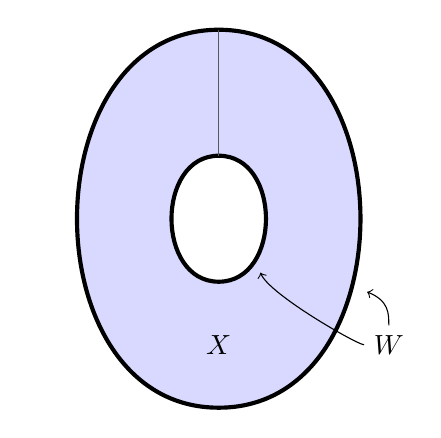
\begin{tikzpicture}[scale=.8, fill=blue!15!white]
\fill (0,1) .. controls +(-1,0) and +(-1,0) .. (0,-1)
		.. controls +(1,0) and +(1,0) .. (0,1) -- (0,3)
		.. controls +(3,0) and +(3,0) .. (0,-3)
		.. controls +(-3,0) and +(-3,0) .. (0,3) -- cycle;
\draw[line width=1.5pt] (0,1) .. controls +(-1,0) and +(-1,0) .. (0,-1)
		.. controls +(1,0) and +(1,0) .. (0,1);
\draw[line width=1.5pt] (0,3) .. controls +(3,0) and +(3,0) .. (0,-3)
		.. controls +(-3,0) and +(-3,0) .. (0,3);
\draw[line width=.5pt, black!65!white] (0,1) -- (0,3);
\node at (0,-2) {$X\sgl$};
\node (W) at (2.7,-2) {$W\sgl$};
\node (we1) at (2.2,-1.1) {};
\node (we2) at (.6,-.7) {};
\draw[->] (W) .. controls +(0,.5) and +(.5,-.2) .. (we1);
\draw[->] (W) .. controls +(-.5,0) and +(.2,-.5) .. (we2);
\end{tikzpicture}
};


\draw[->, red!50!green, line width=2pt] (A) -- node[above, black] {glue} (B);

\end{tikzpicture}
\end{center}
\caption{Gluing with corners}
\label{fig:gluing-with-corners}
\end{figure}
Note that $\bd X\sgl = W\sgl$, where $W\sgl$ denotes $W$ glued to itself
(without corners) along two copies of $\bd Y$.
Let $c\sgl \in \cC_{k-1}(W\sgl)$ be a be a splittable field on $W\sgl$ and let
$c \in \cC_{k-1}(W)$ be the cut open version of $c\sgl$.
Let $\cC^c_k(X)$ denote the subset of $\cC(X)$ which restricts to $c$ on $W$.
(This restriction map uses the gluing without corners map above.)
Using the boundary restriction and gluing without corners maps, 
we get two maps $\cC^c_k(X) \to \cC(Y)$, corresponding to the two
copies of $Y$ in $\bd X$.
Let $\Eq^c_Y(\cC_k(X))$ denote the equalizer of these two maps.
Then (here's the axiom/definition part) there is an injective ``gluing" map
\[
	\Eq^c_Y(\cC_k(X)) \hookrightarrow \cC_k(X\sgl, c\sgl) ,
\]
and this gluing map is compatible with all of the above structure (actions
of homeomorphisms, boundary restrictions, disjoint union).
Furthermore, up to homeomorphisms of $X\sgl$ isotopic to the identity
and collaring maps,
the gluing map is surjective.
We say that fields in the image of the gluing map
are transverse to $Y$ or splittable along $Y$.
\item Product fields.
There are maps $\cC_{k-1}(Y) \to \cC_k(Y \times I)$, denoted
$c \mapsto c\times I$.
These maps comprise a natural transformation of functors, and commute appropriately
with all the structure maps above (disjoint union, boundary restriction, etc.).
Furthermore, if $f: Y\times I \to Y\times I$ is a fiber-preserving homeomorphism
covering $\bar{f}:Y\to Y$, then $f(c\times I) = \bar{f}(c)\times I$.
\end{enumerate}

There are two notations we commonly use for gluing.
One is 
\[
	x\sgl \deq \gl(x) \in \cC(X\sgl) , 
\]
for $x\in\cC(X)$.
The other is
\[
	x_1\bullet x_2 \deq \gl(x_1\otimes x_2) \in \cC(X\sgl) , 
\]
in the case that $X = X_1 \du X_2$, with $x_i \in \cC(X_i)$.

\medskip


Let $M$ be an $n$-manifold and $Y \subset \bd M$ be a codimension zero submanifold
of $\bd M$.
Let $M \cup (Y\times I)$ denote $M$ glued to $Y\times I$ along $Y$.
Extend the product structure on $Y\times I$ to a bicollar neighborhood of 
$Y$ inside $M \cup (Y\times I)$.
We call a homeomorphism
\[
	f: M \cup (Y\times I) \to M
\]
a {\it collaring homeomorphism} if $f$ is the identity outside of the bicollar
and $f$ preserves the fibers of the bicollar.

Using the functoriality and product field properties above, together
with collaring homeomorphisms, we can define 
{\it collar maps} $\cC(M)\to \cC(M)$.
Let $M$ and $Y \sub \bd M$ be as above.
Let $x \in \cC(M)$ be a field on $M$ and such that $\bd x$ is splittable along $\bd Y$.
Let $c$ be $x$ restricted to $Y$.
Then we have the glued field $x \bullet (c\times I)$ on $M \cup (Y\times I)$.
Let $f: M \cup (Y\times I) \to M$ be a collaring homeomorphism.
Then we call the map $x \mapsto f(x \bullet (c\times I))$ a {\it collar map}.

We call the equivalence relation generated by collar maps and
homeomorphisms isotopic to the identity {\it extended isotopy}, since the collar maps
can be thought of (informally) as the limit of homeomorphisms
which expand an infinitesimally thin collar neighborhood of $Y$ to a thicker
collar neighborhood.




\subsection{Systems of fields from \texorpdfstring{$n$}{n}-categories}
\label{sec:example:traditional-n-categories(fields)}
We now describe in more detail Example \ref{ex:traditional-n-categories(fields)}, 
systems of fields coming from embedded cell complexes labeled
by $n$-category morphisms.

Given an $n$-category $C$ with the right sort of duality
(e.g. a pivotal 2-category, *-1-category),
we can construct a system of fields as follows.
Roughly speaking, $\cC(X)$ will the set of all embedded cell complexes in $X$
with codimension $i$ cells labeled by $i$-morphisms of $C$.
We'll spell this out for $n=1,2$ and then describe the general case.

This way of decorating an $n$-manifold with an $n$-category is sometimes referred to
as a ``string diagram".
It can be thought of as (geometrically) dual to a pasting diagram.
One of the advantages of string diagrams over pasting diagrams is that one has more
flexibility in slicing them up in various ways.
In addition, string diagrams are traditional in quantum topology.
The diagrams predate by many years the terms ``string diagram" and 
``quantum topology", e.g. \cite{MR0281657,MR776784} % both penrose

If $X$ has boundary, we require that the cell decompositions are in general
position with respect to the boundary --- the boundary intersects each cell
transversely, so cells meeting the boundary are mere half-cells.
Put another way, the cell decompositions we consider are dual to standard cell
decompositions of $X$.

We will always assume that our $n$-categories have linear $n$-morphisms.

\nn{need to replace ``cell decomposition" below with something looser.  not sure what to call it.
maybe ``nice stratification"??  the link of each piece of each stratum should be a cell decomposition of
a sphere, but that's probably all we need.  or maybe refineable to a cell decomp?}

For $n=1$, a field on a 0-manifold $P$ is a labeling of each point of $P$ with
an object (0-morphism) of the 1-category $C$.
A field on a 1-manifold $S$ consists of
\begin{itemize}
    \item a cell decomposition of $S$ (equivalently, a finite collection
of points in the interior of $S$);
    \item a labeling of each 1-cell (and each half 1-cell adjacent to $\bd S$)
by an object (0-morphism) of $C$;
    \item a transverse orientation of each 0-cell, thought of as a choice of
``domain" and ``range" for the two adjacent 1-cells; and
    \item a labeling of each 0-cell by a 1-morphism of $C$, with
domain and range determined by the transverse orientation and the labelings of the 1-cells.
\end{itemize}

We want fields on 1-manifolds to be enriched over Vect, so we also allow formal linear combinations
of the above fields on a 1-manifold $X$ so long as these fields restrict to the same field on $\bd X$.

In addition, we mod out by the relation which replaces
a 1-morphism label $a$ of a 0-cell $p$ with $a^*$ and reverse the transverse orientation of $p$.

If $C$ is a *-algebra (i.e. if $C$ has only one 0-morphism) we can ignore the labels
of 1-cells, so a field on a 1-manifold $S$ is a finite collection of points in the
interior of $S$, each transversely oriented and each labeled by an element (1-morphism)
of the algebra.

\medskip

For $n=2$, fields are just the sort of pictures based on 2-categories (e.g.\ tensor categories)
that are common in the literature.
We describe these carefully here.

A field on a 0-manifold $P$ is a labeling of each point of $P$ with
an object of the 2-category $C$.
A field of a 1-manifold is defined as in the $n=1$ case, using the 0- and 1-morphisms of $C$.
A field on a 2-manifold $Y$ consists of
\begin{itemize}
    \item a cell decomposition of $Y$ (equivalently, a graph embedded in $Y$ such
that each component of the complement is homeomorphic to a disk);
    \item a labeling of each 2-cell (and each partial 2-cell adjacent to $\bd Y$)
by a 0-morphism of $C$;
    \item a transverse orientation of each 1-cell, thought of as a choice of
``domain" and ``range" for the two adjacent 2-cells;
    \item a labeling of each 1-cell by a 1-morphism of $C$, with
domain and range determined by the transverse orientation of the 1-cell
and the labelings of the 2-cells;
    \item for each 0-cell, a homeomorphism of the boundary $R$ of a small neighborhood
of the 0-cell to $S^1$ such that the intersections of the 1-cells with $R$ are not mapped
to $\pm 1 \in S^1$
(this amounts to splitting of the link of the 0-cell into domain and range); and
    \item a labeling of each 0-cell by a 2-morphism of $C$, with domain and range
determined by the labelings of the 1-cells and the parameterizations of the previous
bullet.
\end{itemize}

As in the $n=1$ case, we allow formal linear combinations of fields on 2-manifolds, 
so long as their restrictions to the boundary coincide.

In addition, we regard the labelings as being equivariant with respect to the * structure
on 1-morphisms and pivotal structure on 2-morphisms.
That is, we mod out by the relation which flips the transverse orientation of a 1-cell 
and replaces its label $a$ by $a^*$, as well as the relation which changes the parameterization of the link
of a 0-cell and replaces its label by the appropriate pivotal conjugate.

\medskip

For general $n$, a field on a $k$-manifold $X^k$ consists of
\begin{itemize}
    \item A cell decomposition of $X$;
    \item an explicit general position homeomorphism from the link of each $j$-cell
to the boundary of the standard $(k-j)$-dimensional bihedron; and
    \item a labeling of each $j$-cell by a $(k-j)$-dimensional morphism of $C$, with
domain and range determined by the labelings of the link of $j$-cell.
\end{itemize}



\subsection{Local relations}
\label{sec:local-relations}

For convenience we assume that fields are enriched over Vect.

Local relations are subspaces $U(B; c)\sub \cC(B; c)$ of the fields on balls which form an ideal under gluing.
Again, we give the examples first.

\addtocounter{prop}{-2}
\begin{example}[contd.]
For maps into spaces, $U(B; c)$ is generated by fields of the form $a-b \in \lf(B; c)$,
where $a$ and $b$ are maps (fields) which are homotopic rel boundary.
\end{example}

\begin{example}[contd.]
For $n$-category pictures, $U(B; c)$ is equal to the kernel of the evaluation map
$\lf(B; c) \to \mor(c', c'')$, where $(c', c'')$ is some (any) division of $c$ into
domain and range.
\end{example}

These motivate the following definition.

\begin{defn}
A {\it local relation} is a collection subspaces $U(B; c) \sub \lf(B; c)$,
for all $n$-manifolds $B$ which are
homeomorphic to the standard $n$-ball and all $c \in \cC(\bd B)$, 
satisfying the following properties.
\begin{enumerate}
\item Functoriality: 
$f(U(B; c)) = U(B', f(c))$ for all homeomorphisms $f: B \to B'$
\item Local relations imply extended isotopy: 
if $x, y \in \cC(B; c)$ and $x$ is extended isotopic 
to $y$, then $x-y \in U(B; c)$.
\item Ideal with respect to gluing:
if $B = B' \cup B''$, $x\in U(B')$, and $r\in \cC(B'')$, then $x\bullet r \in U(B)$
\end{enumerate}
\end{defn}
See \cite{kw:tqft} for further details.


\subsection{Constructing a TQFT}
\label{sec:constructing-a-tqft}

In this subsection we briefly review the construction of a TQFT from a system of fields and local relations.
As usual, see \cite{kw:tqft} for more details.

We can think of a path integral $Z(W)$ of an $n+1$-manifold 
(which we're not defining in this context; this is just motivation) as assigning to each
boundary condition $x\in \cC(\bd W)$ a complex number $Z(W)(x)$.
In other words, $Z(W)$ lies in $\c^{\lf(\bd W)}$, the vector space of linear
maps $\lf(\bd W)\to \c$.

The locality of the TQFT implies that $Z(W)$ in fact lies in a subspace
$Z(\bd W) \sub \c^{\lf(\bd W)}$ defined by local projections.
The linear dual to this subspace, $A(\bd W) = Z(\bd W)^*$,
can be thought of as finite linear combinations of fields modulo local relations.
(In other words, $A(\bd W)$ is a sort of generalized skein module.)
This is the motivation behind the definition of fields and local relations above.

In more detail, let $X$ be an $n$-manifold.
%To harmonize notation with the next section, 
%let $\bc_0(X)$ be the vector space of finite linear combinations of fields on $X$, so
%$\bc_0(X) = \lf(X)$.
\begin{defn}
\label{defn:TQFT-invariant}
The TQFT invariant of $X$ associated to a system of fields $\cC$ and local relations $U$ is 
	$$A(X) \deq \lf(X) / U(X),$$
where $U(X) \sub \lf(X)$ is the space of local relations in $\lf(X)$:
$U(X)$ is generated by fields of the form $u\bullet r$, where
$u\in U(B)$ for some embedded $n$-ball $B\sub X$ and $r\in \cC(X\setmin B)$.
\end{defn}
The blob complex, defined in the next section, 
is in some sense the derived version of $A(X)$.
If $X$ has boundary we can similarly define $A(X; c)$ for each 
boundary condition $c\in\cC(\bd X)$.

The above construction can be extended to higher codimensions, assigning
a $k$-category $A(Y)$ to an $n{-}k$-manifold $Y$, for $0 \le k \le n$.
These invariants fit together via actions and gluing formulas.
We describe only the case $k=1$ below.
The construction of the $n{+}1$-dimensional part of the theory (the path integral) 
requires that the starting data (fields and local relations) satisfy additional
conditions.
We do not assume these conditions here, so when we say ``TQFT" we mean a decapitated TQFT
that lacks its $n{+}1$-dimensional part. 
Such a ``decapitated'' TQFT is sometimes also called an $n+\epsilon$ or 
$n+\frac{1}{2}$ dimensional TQFT, referring to the fact that it assigns maps to 
mapping cylinders between $n$-manifolds, but nothing to arbitrary $n{+}1$-manifolds.

Let $Y$ be an $n{-}1$-manifold.
Define a linear 1-category $A(Y)$ as follows.
The set of objects of $A(Y)$ is $\cC(Y)$.
The morphisms from $a$ to $b$ are $A(Y\times I; a, b)$, 
where $a$ and $b$ label the two boundary components of the cylinder $Y\times I$.
Composition is given by gluing of cylinders.

Let $X$ be an $n$-manifold with boundary and consider the collection of vector spaces
$A(X; -) \deq \{A(X; c)\}$ where $c$ ranges through $\cC(\bd X)$.
This collection of vector spaces affords a representation of the category $A(\bd X)$, where
the action is given by gluing a collar $\bd X\times I$ to $X$.

Given a splitting $X = X_1 \cup_Y X_2$ of a closed $n$-manifold $X$ along an $n{-}1$-manifold $Y$,
we have left and right actions of $A(Y)$ on $A(X_1; -)$ and $A(X_2; -)$.
The gluing theorem for $n$-manifolds states that there is a natural isomorphism
\[
	A(X) \cong A(X_1; -) \otimes_{A(Y)} A(X_2; -) .
\]
A proof of this gluing formula appears in \cite{kw:tqft}, but it also becomes a 
special case of Theorem \ref{thm:gluing} by taking $0$-th homology.
